% Authors: Son Tran, Naomi Sagan, Taejin Hwang
% Emails: sontran@berkeley.edu, naomi.sagan@berkeley.edu, taejin@berkeley.edu

\qns{Change of Coordinates}

Many engineering problems can be difficult to solve in its standard xyz coordinates, but may be much easier in a different coordinate system.
In this set, we will review the process of \textbf{change of basis} between coordinate systems.
Remember that a \emph{change of basis} can be represented by a invertible, square matrix. \vskip 1pt
Let's first start with an example:
Consider the vector $\vec{x} = \begin{bmatrix} x_1 \\ x_2 \end{bmatrix}.$ 
When we write a vector in this form, we are implicitly representing it with the \textbf{standard basis} for $\R^{2}$, $\vec{e_1} = \begin{bmatrix} 1 \\ 0 \end{bmatrix}$ and $\vec{e_2} = \begin{bmatrix} 0 \\ 1 \end{bmatrix}.$ \vspace{1em} 
This means that we can write $\vec{x}$ as a linear combination using standard basis vectors $\vec{x} = x_1\vec{e_1} + x_2\vec{e_2}$. \vspace {1em} 
Now, what if we want to represent $\vec{x}$ as a linear combination of another set of basis vectors, say $\vec{v_1} = \begin{bmatrix} 1 \\ 1 \end{bmatrix}$ and $\vec{v_2} = \begin{bmatrix} 0 \\ -1 \end{bmatrix}?$ \vskip 1pt
This means that we need to find scalars $\alpha_{1}$ and $\alpha_{2}$ such that $\vec{x} = \alpha_1 \vec{v_1} + \alpha_2 \vec{v_2}$.
We can write this equation in matrix form:
\[
  \begin{bmatrix}
    | & | \\
    \vec{v_1} & \vec{v_2} \\
    | & |
  \end{bmatrix}
  \begin{bmatrix} \alpha_1 \\ \alpha_2 \end{bmatrix} = \begin{bmatrix} x_1 \\ x_2 \end{bmatrix}
.\]

Or equivalently:
\[
  \begin{bmatrix}
    1 & 0 \\
    1 & -1
  \end{bmatrix}
  \begin{bmatrix} \alpha_1 \\ \alpha_2 \end{bmatrix} = \begin{bmatrix} x_1 \\ x_2 \end{bmatrix}
.\]
Thus we can find $\alpha_1$ and $\alpha_2$ by solving a system of linear equations as seen in 16A. \\
These scalars $\alpha_1$ and $\alpha_2$ are called the coordinates of $\vec{x}$ \textbf{in the basis} $S = \{\vec{v_1}, \vec{v_2} \}.$

For the following problems, we will look at a vector $\vec{x}$ currently in the standard basis 
and its representation in a different basis: $S = \{\vec{v_1}, \vec{v_2} \}.$ \vskip 4pt
We will refer to the vector $\vec{x}$ using coordinates from the basis $S$ as $[\vec{x}]_S.$ In other words, \vskip 3pt 
if $\vec{x} = \begin{bmatrix} x_1 \\ x_2 \end{bmatrix},$ and $[\vec{x}]_S = \begin{bmatrix} \alpha_1 \\ \alpha_2 \end{bmatrix},$ then $\vec{x} = x_1 \vec{e_1} + x_2 \vec{e_2}$ or $\vec{x} = \alpha_1 \vec{v_1} + \alpha_2 \vec{v_2}.$

\begin{enumerate}
  % Part(a)
  \qitem Now let's say we have a vector that is originally using coordinates from the basis S. 
  That is $[\vec{x}]_S = \begin{bmatrix} 3 \\ 3 \end{bmatrix}.$ We are told that the basis S is:
  \begin{gather*}
    \vec{v_1} =
    \begin{bmatrix}
      1 \\
      1
    \end{bmatrix},
    \vec{v_2} = \begin{bmatrix}
      1 \\
      -1
    \end{bmatrix}
  \end{gather*}
  What equation gives the coordinates of $\vec{x}$ in the standard basis?

  % Part(a) solution
  \sol{
    Since the vector $\vec{x}$ is currently written in coordinates using the basis, $S = \{\vec{v_1}, \vec{v_2} \},$
    we know that $\vec{x} = 3 \begin{bmatrix} 1 \\ 1 \end{bmatrix} + 3 \begin{bmatrix} 1 \\ -1 \end{bmatrix} = V [\vec{x}]_S$
    where $V$ is the matrix $\begin{bmatrix} 1 & 1 \\ 1 & -1 \end{bmatrix}.$ Therefore,
    $$
    \vec{x} =
    \begin{bmatrix}
      1 & 1 \\
      1 & -1
    \end{bmatrix}
    \begin{bmatrix}
      3 \\
      3
    \end{bmatrix}
    $$
  }

  % Part(b)
  \qitem Let $\vec{x} = \begin{bmatrix} 2 \\ -1 \end{bmatrix}$. What equation gives the coordinates of $\vec{x}$ in the basis S? 
  Try to express your answer in matrix-vector form. No need to do the full calculation.
  \begin{gather*}
    \vec{v_1} =
    \begin{bmatrix}
      4 \\
      -2
    \end{bmatrix},
    \vec{v_2} = \begin{bmatrix}
      -3 \\
      -3
    \end{bmatrix}
  \end{gather*}
  What equation gives the coordinates of $\vec{v}$ in the standard basis?

  % Part(b) solution
  \sol {
    If we denote the vector in the new basis as $[\vec{x}]_S = \begin{bmatrix} \alpha_1 \\ \alpha_2 \end{bmatrix}$, then we can write out the following equation: $\vec{x} = \alpha_1 \vec{v_1} + \alpha_2 \vec{v_2} = V [\vec{x}]_S$ where V is the same matrix used in the previous part. Then it follows that $[\vec{x}]_S = V^{-1} \vec{x}.$
  }

  \end{enumerate}

  Now that we've had some mechanical practice, we'll look at the representation of linear operators through different bases. 
  For a linear transformation, we can represent the input-output relationship with the matrix vector equation:
  $\vec{y} = A \vec{x}$ where $\vec{x}$ is the input, and $\vec{y}$ is the output vector.
  In this question we will look at how the linear operator represented by the matrix $A$ looks in a \textit{different basis} $S.$
  Remember that the vector $\vec{x}$ is implicitly written in the \textbf{standard basis} while the vector $[\vec{x}]_S$ is a vector using coordinates from the \textbf{S-basis.}

  \begin{enumerate}[resume]
  %part c
  \qitem Let $[\vec{x}]_S$ be a vector using $S$ coordinates, and $V$ be a change of coordinates matrix from the $S$-basis to the standard basis. \\
  How can we represent $[\vec{x}]_S$ in terms of $\vec{x}$ and $V?$
  \sol {
    We are given a matrix $V$ that converts $S$ coordinates to standard coordinates. 
    This means that $V^{-1}$ will be the matrix that converts standard coordinates to the $S$ coordinates.
    Therefore, in order to get $[\vec{x}]_S$ we multiply $V^{-1}$ with $\vec{x},$ to get
    $V^{-1} \vec{x} = [\vec{x}]_S.$
  }

  % Part(d)
  \qitem Now suppose we have another basis $R = \{w_1, .. , w_n\}$ and the change of basis from $R$ to $S$ is represented by the matrix $W.$ This means that if we have a vector $[\vec{x}]_R$ in R-coordinates, to get the coordinate representation in S-coordinates, $[\vec{x}]_S = W[\vec{x}]_R.$ What would the change of basis matrix that takes a vector in $R$ coordinates and outputs a vector in standard coordinates look like?
  \sol {
    We want to get represent the vector $\vec{x}$ in standard coordinates.
    We are looking for a matrix $U$ such that
    $$\vec{x} = U [\vec{x}]_R.$$
    We currently know that in order to go from S-coordinates to standard, we must multiply by the matrix $V.$
    $$\vec{x} = V [\vec{x}]_S.$$
    We also know that to go from R-coordinates to S-coordinates, we must multiply by the matrix $W.$
    $$[\vec{x}]_S = W [\vec{x}]_R.$$
    Therefore, by substituting $[\vec{x}]_S,$ we see that
    $$\vec{x} = V W [\vec{x}]_R.$$
    It follows that the matrix $U = VW.$
  }

  % Part(d)
  \qitem Now let $B$ be a linear operator in $\beta$ coordinates. This means that it will take in a vector $[\vec{x}]_\beta$ as an input and output $[\vec{y}]_\beta.$ Given a vector $\vec{x}$ in standard coordinates, why can't we multiply $B \vec{x}$ to get the output $\vec{y}$ in standard coordinates?

  \sol{
    The transformation $B$ "lives" in a different world. It can only accept vectors in $\beta$ coordinates as inputs. 
    Therefore, in order to solve this, we must convert $\vec{x}$ into $\beta$ coordinates.
  }

  % Part(e)
  \qitem Using our $V$ matrix given above, as the change of coordinates matrix from $S \to \beta,$ how can we describe the linear operator $B$ in standard coordinates, that is if $\vec{y} = A \vec{x},$ what is $A$ in the standard basis?

  \sol {
    There will be two main issues we need to address in this question. First off, we need a $\beta$ coordinate input. Secondly, the output of the $B$ matrix is in $\beta$ coordinates, and we will need to convert that back to standard coordinates. 

    Therefore, we take the following steps.

    1. Let's first make our input into $B$ in $\beta$ coordinates. 
    $$\text{Let } V \vec{v} = \vec{x}.$$
    2. Now if we input $\vec{v}$ we will get some output:
    $$\vec{w} = B \vec{v}.$$
    3. However, $\vec{w}$ is in $\beta$ coordinates, so we must convert back to standard coordinates using $V^{-1}.$
    $$V^{-1} \vec{y} =  \vec{w}$$
    4. Cascading all of our matrix multiplications, we end up with:
    $$\vec{y} = V B V^{-1} \vec{x}.$$
    Therefore, we can see that $A = V B V^{-1} .$

    The following can also be represented in this state diagram: 

    Note that when cascading transformations, we apply them to the \textbf{left} of the existing transformation.

    \begin{figure}[H]
      \centering
      \begin{tikzpicture}[node distance = 2cm, thick]%
        \node (1) {$\vec{x}$};
        \node (2) [right=of 1] {$\vec{y}$};
        \node (3) [below=of 2] {$\vec{w}$};
        \node (4) [below=of 1] {$\vec{v}$};
        \draw[->] (1) -- node [midway,above] {$A$} (2);
        \draw[->] (1.240) -- node [midway,left]{$V^{-1}$} (4.120);
        \draw[->] (4.60) -- node [midway,right]{$V$} (1.300);
        \draw[->] (2.300) -- node [midway,right]{$V^{-1}$} (3.60);
        \draw[->] (3.120) -- node [midway,left]{$V$} (2.240);
        \draw[->] (4) -- node [midway,below] {$B$} (3);
      \end{tikzpicture}%
    \end{figure}
  }
  % % Part(c) solution
  % \sol{
  %   Start by writing $\vec{x_1}$ in terms of $\vec{z_1}$:
  %   $$ \vec{x_1} = V \vec{z_1} $$
  %   Then, apply the transformation $A$ to $\vec{x_1}$, substituting $V \vec{z_1}$ for $\vec{x_1}$:
  %   $$ \vec{x_2} = A V \vec{x_1} $$
  %   Finally, left-multiply both sides by $V^{-1}$ to change $\vec{x_2}$ to the eigenbasis:
  %   $$ \vec{z_2} = V^{-1} \vec{x_2} = V^{-1} A V \vec{z_1} $$

  %   $$A' = V^{-1} A V =
  %   \begin{bmatrix}
  %     1 & 1 \\
  %     -2 & 1
  %   \end{bmatrix}^{-1}
  %   \begin{bmatrix}
  %     3 & -1 \\
  %     -2 & 4
  %   \end{bmatrix}
  %   \begin{bmatrix}
  %     1 & 1 \\
  %     -2 & 1
  %   \end{bmatrix}
  %   $$

  %   $A'$ represents the transformation $A$ in the eigenbasis of $A$, so we know that $A'$ is the diagonal matrix:
  %   $$ A' =
  %   \begin{bmatrix}
  %     \lambda_1 & 0 \\
  %     0 & \lambda_2
  %   \end{bmatrix} =
  %   \begin{bmatrix}
  %     5 & 0 \\
  %     0 & 2
  %   \end{bmatrix} $$

  %   In general, suppose we have a linear transformation $T$ represented by a $n \times n$ matrix that transforms $\vec{u} \in \R^{n}$ to $\vec{v} \in \R^{n}$:
  %   \[
  %     \vec{v} = T\vec{u}
  %   .\]
  %   Suppose we have a basis vectors $\vec{a_1}, \cdots, \vec{a_n} \in \R^{n}$, and the vectors $\vec{u}, \vec{v}$ above are represented in this basis:
  %   \[
  %     \begin{aligned}
  %       \vec{u_a} &= u_{a_1}\vec{a_1} + \cdots + u_{a_n}\vec{a_n} \\
  %       \vec{v_a} &= v_{a_1}\vec{a_1} + \cdots + v_{a_n}\vec{a_n}.
  %     \end{aligned}
  %   \]
  %   Thus we have
  %   \[
  %     \begin{aligned}
  %       T\vec{u}          &= \vec{v} \\
  %       TA\vec{u_a}       &= A\vec{v_a} \\
  %       A^{-1}TA\vec{u_a} &= \vec{v_a}.
  %     \end{aligned}
  %   \]
  %   By pattern matching, we see that if we set $T_a = A^{-1}TA$, we get the relationship $T_a\vec{u_a} = \vec{v_a}$ in the new basis.
  %   The correspondences stated above are all represented in the following diagram:
  %   % \begin{figure}[H]
  %   %   \centering
  %   %   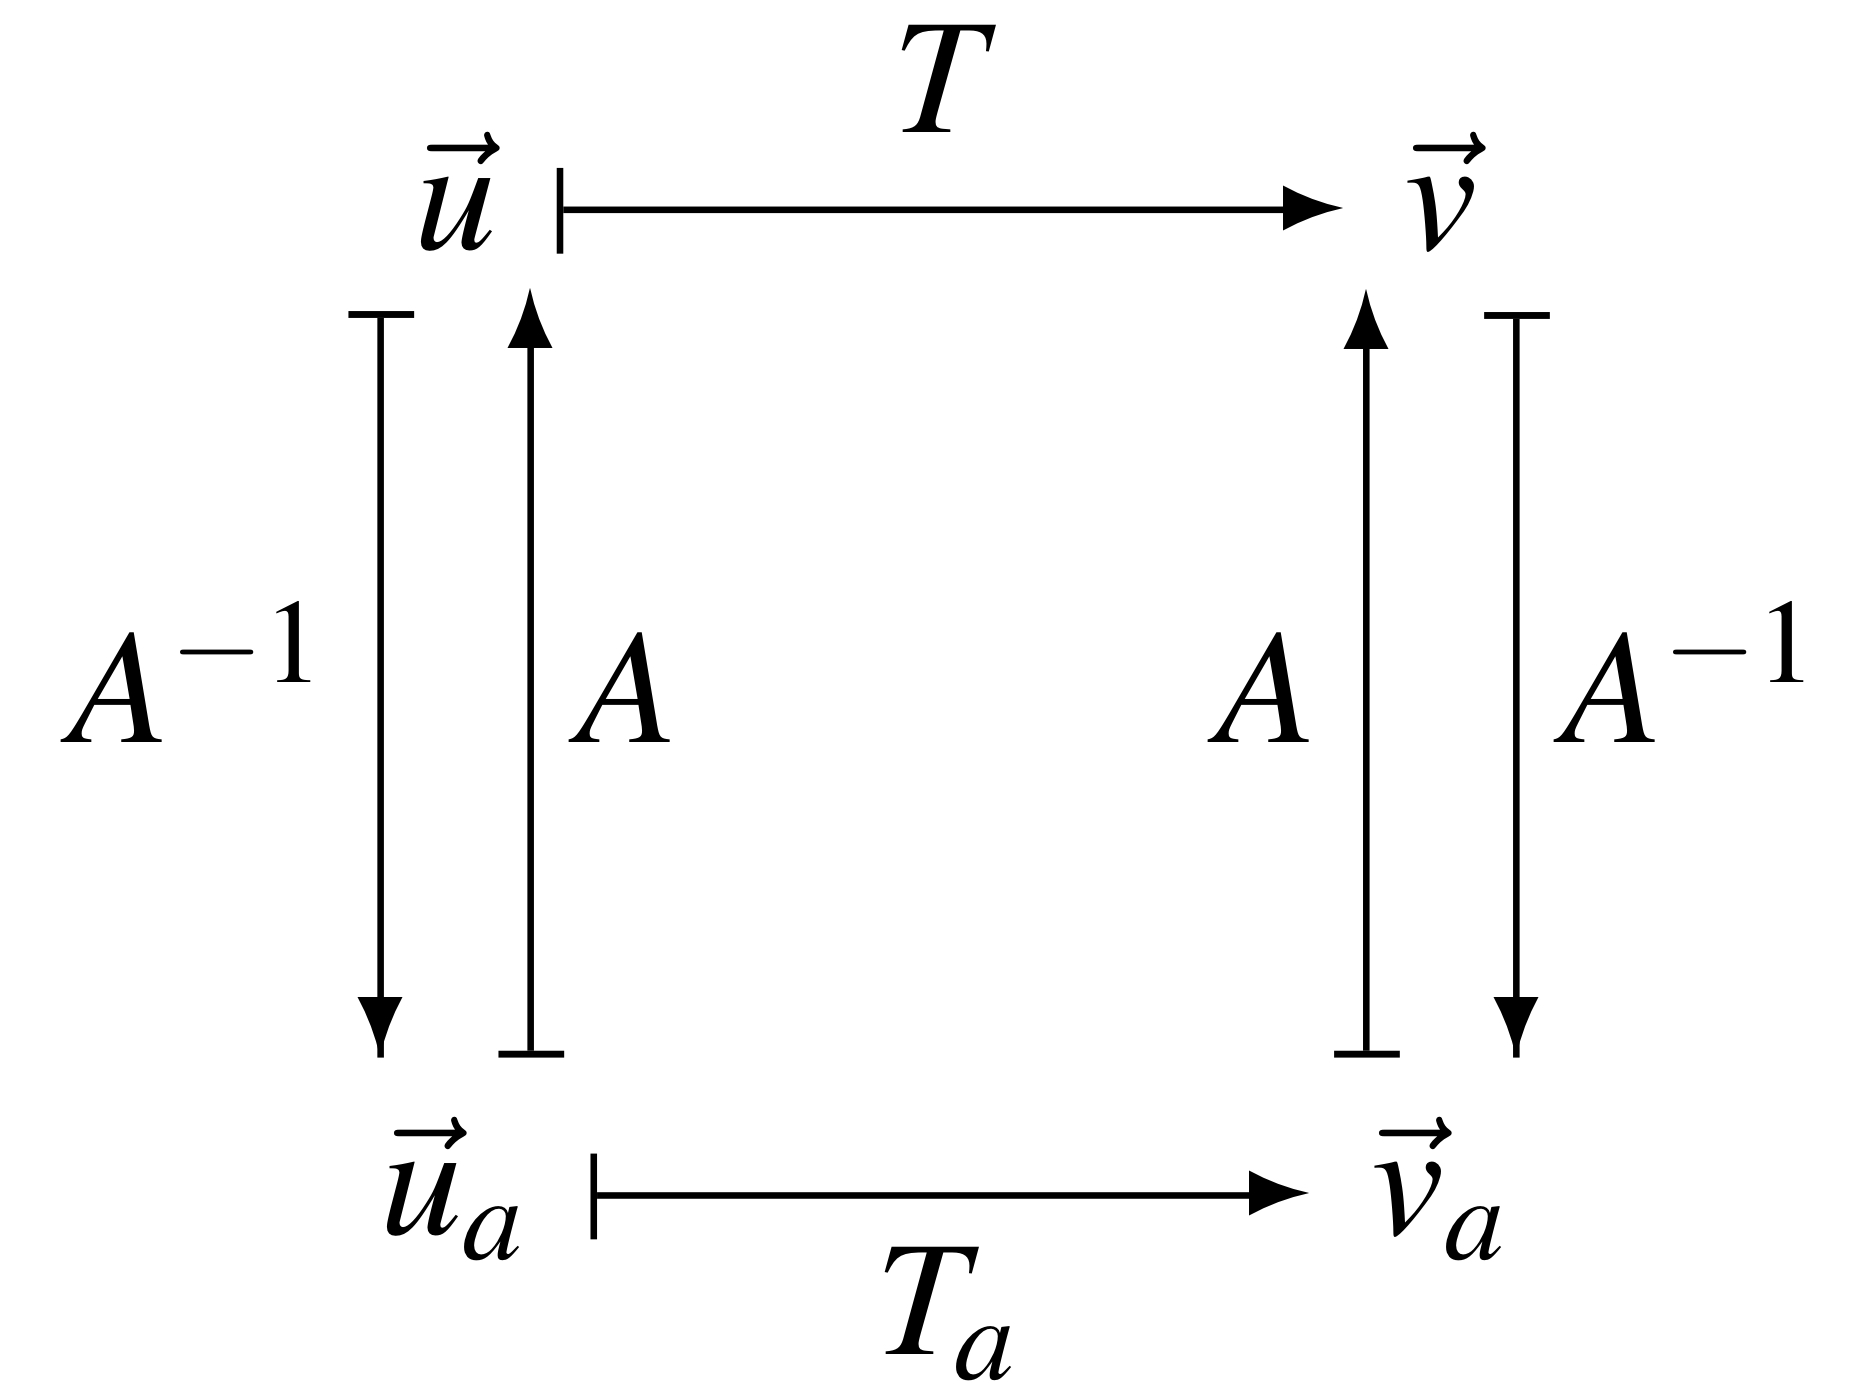
\includegraphics[scale=0.1]{\bank/statespace/figures/change_of_basis.jpg}
  %   % \end{figure}
\end{enumerate}
